\documentclass[../main.tex]{subfiles}
\graphicspath{{\subfix{../../images/}}}
\begin{document}

\chapter{Experimental Methods}\label[chapter]{methods}

\bigskip
\begin{quote}
    \emph{We have some idea as to the intricate design of the puppet and the puppet strings, but we lack insight into the mind of the puppeteer.}
    \raggedleft{
    \begin{spacing}{1.125}
          {--- Emilio Bizzi \& ??? Ajemian} \\ \emph{???, 2020}
    \end{spacing}
    }
\end{quote}

\cleardoublepage

\section{Methodological Aims}\label{methods_aims}

The concept of the experimental setup is shown in \Cref{fig:setup}, where 32 monopolar electrodes are attached to a subject's forearm to record muscle activity. The arm and hand are kinematically constrained in a custom fixture and motor activity is recorded during low-level isometric muscle contractions. The setup circumvents the limb biomechanics by mapping muscle output directly to virtual stimuli shown on a screen. By focusing on low-force, isometric contractions we intend to avoid complications due to artifacts in dynamic, high-force movements.


\section{Recording Setup}\label{hardware}

Describe the experimental setup/environment, what is taking place in each session, protocol, software, hardware, how the signal is captured, physical setup


\begin{figure}
\centering
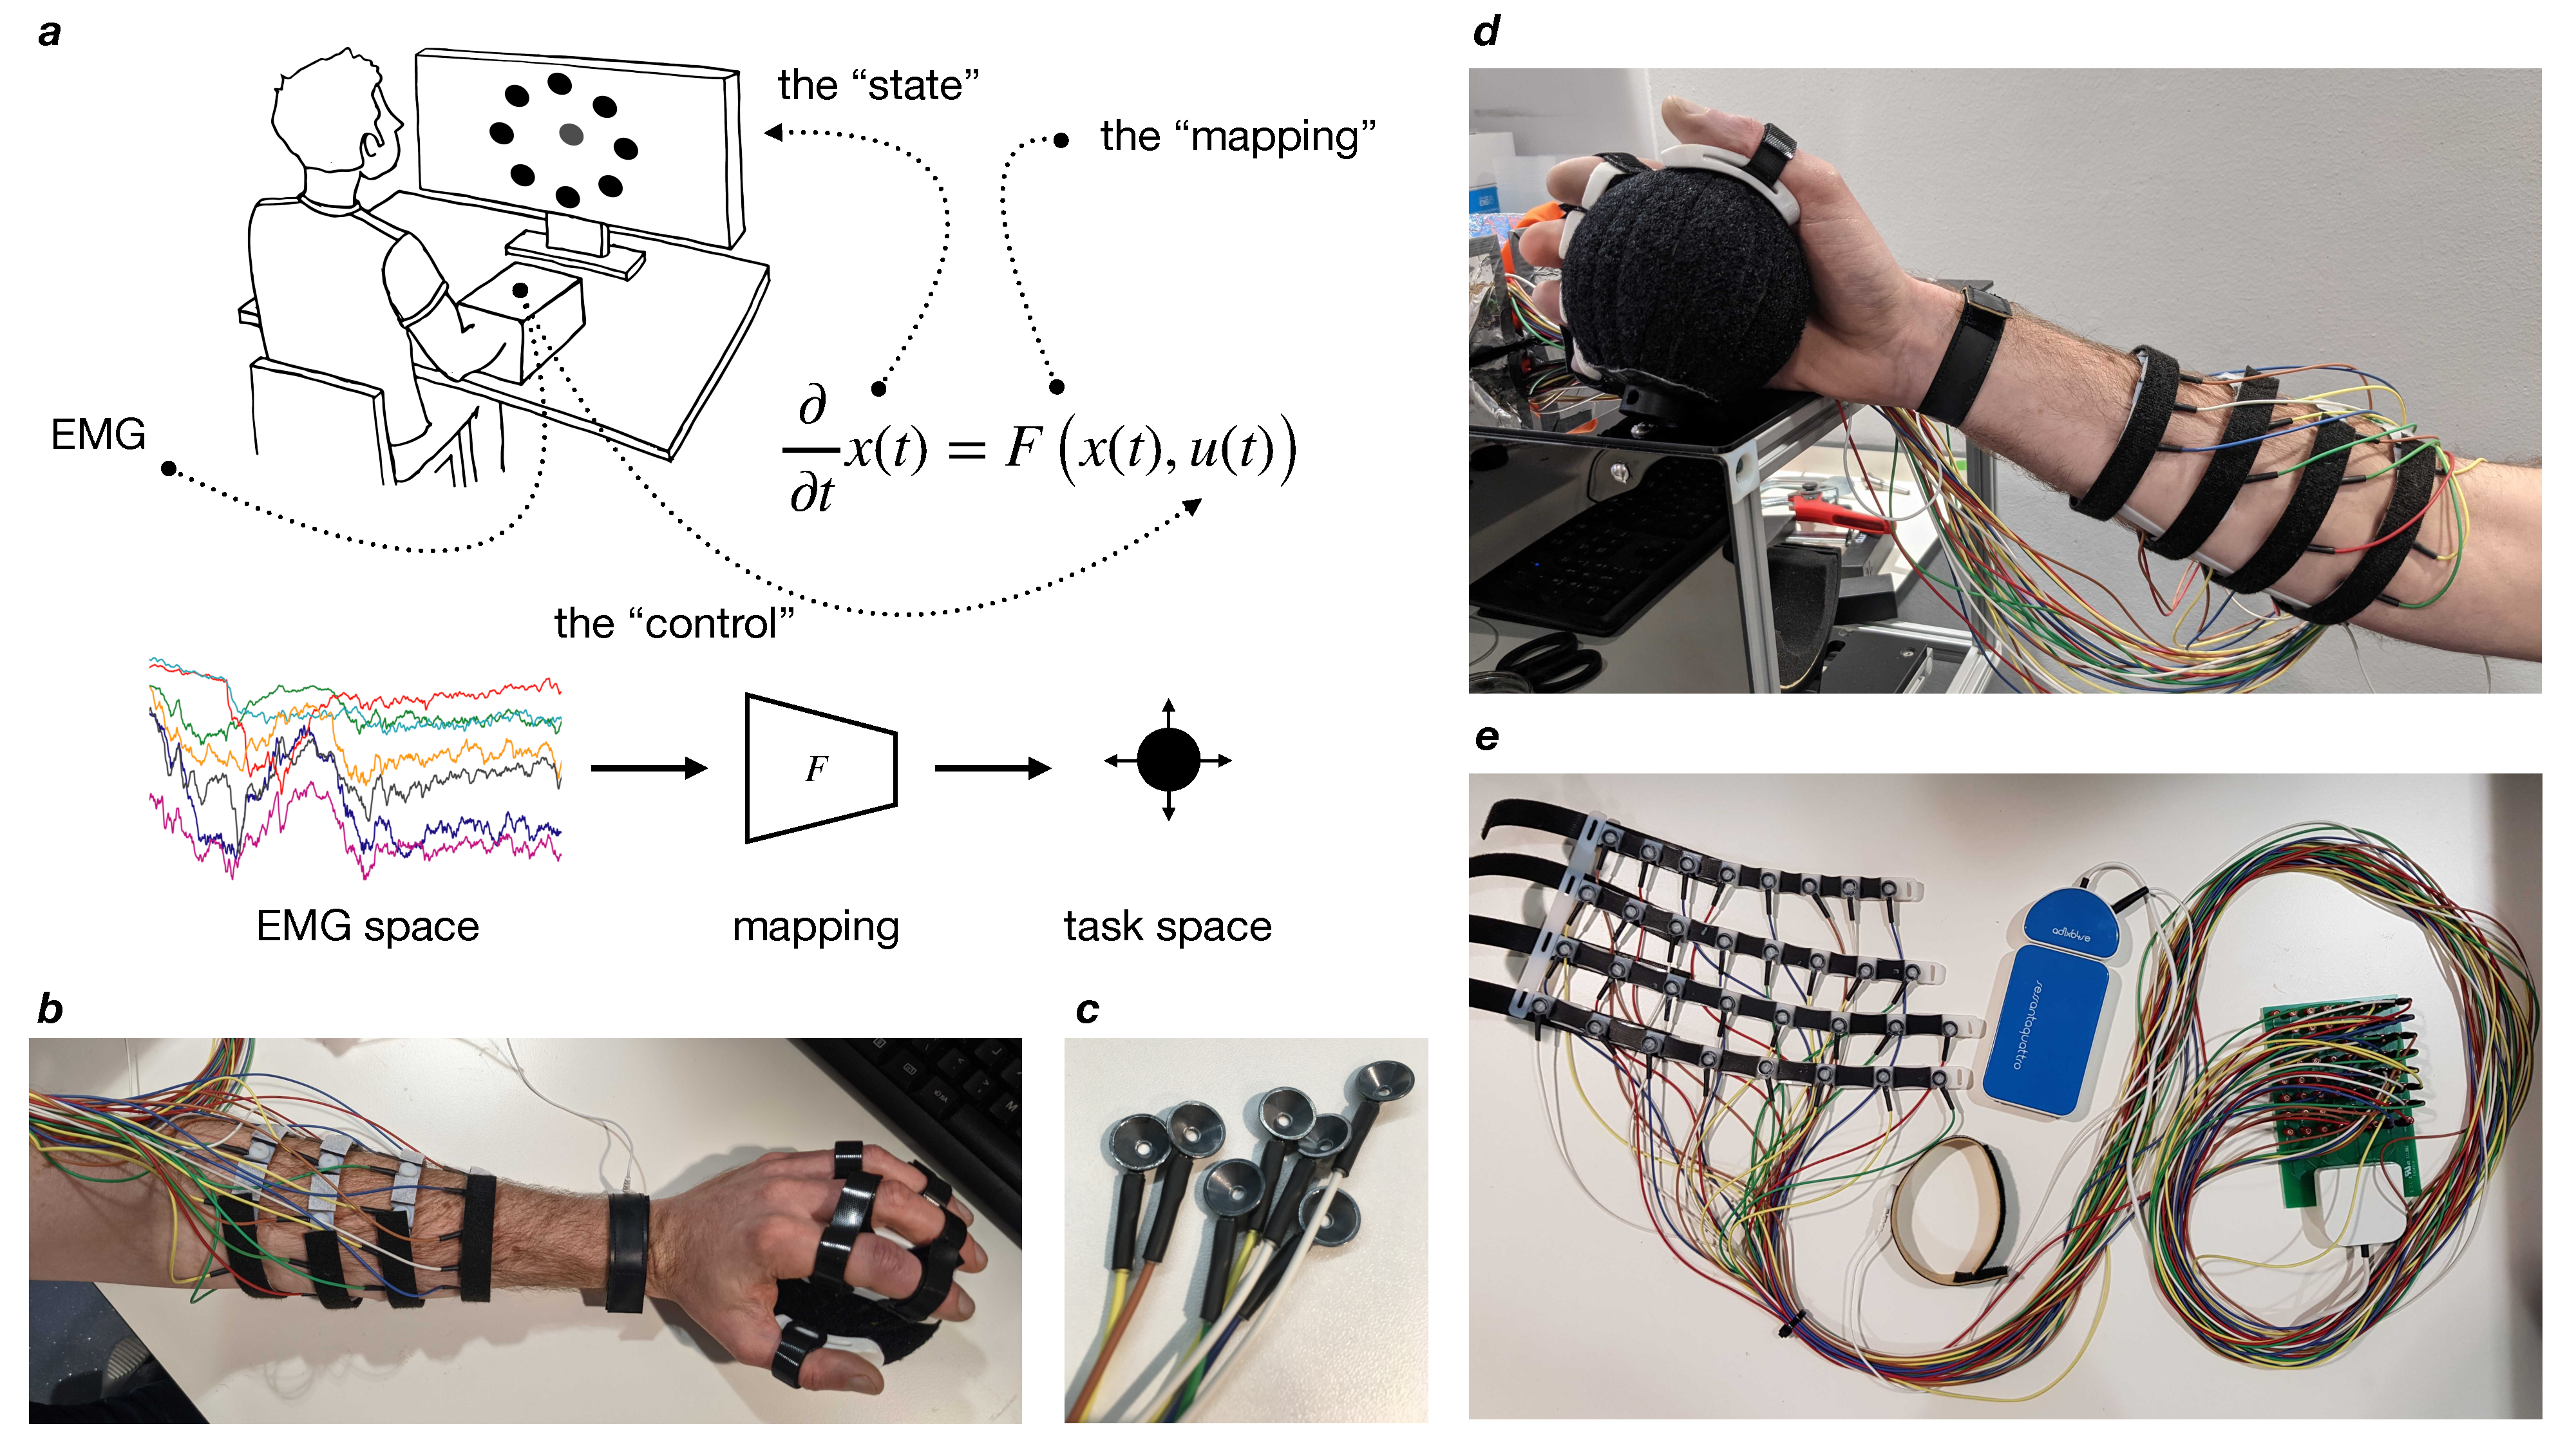
\includegraphics[width=1.0\textwidth]{methods/setup.pdf}
\caption{(a) Graphic depicting the closed-loop EMG interface concept in a center-hold, reach-out type task. The multidimensional EMG signal is transformed online through a mapping $F$ from EMG electrode space to a lower dimensional task space, creating an experimentally controllable redundancy problem for the subject. In experiments shown here the task space is two-dimensional, though the EMG interface can be extended to tasks with higher-dimensional inputs. The subject's arm and hand are constrained during the experiment to ensure isometric contractions. (b) First prototype of custom recording hardware consisting of four bands of eight electrodes each, and a spherical hand constraint. Our recordings are 32 channel monopolar recording with reference electrode at the wrist. (c) Example cup-style monopolar recording electrodes, 5mm in diameter. (d) Side view of the recording hardware. Also pictured is the arm restraint frame to ensure isometric contractions. The frame obscures the subject's arm from view and contains adjustable elbow and wrist rests. (d) Recording hardware shown off the arm with wireless amplifier and connection board.}\label{fig:setup}
\end{figure}

As far as we are aware, this setup is novel in combining a high number of channels with an abstract mapping. Learning experiments have used joint angles and a few muscles (typically movements of the wrist or pairs of thumb and intrinsic hand muscles), but none have taken a data-driven approach in constructing a virtual learning environment in the style of cortical BMI\cite{@BergerDifferencesInAdaptationRates2013a;@Dyson2018;@radhakrishnanLearningNovelMyoelectricControlled2008;@Gallego2017}. Our EMG recording setup is custom-built: the ``Sessantaquattro'' EMG amplifier was acquired from OT Bioelettronica, the electronic connector was designed in-house, the electrodes were acquired from Medkit UK, and the recording software was written in a mixture of Bonsai (C\#) and Python. EMG is acquired at 2kHz sample rate with 24-bit precision. A clip of raw data is shown in \Cref{fig:raw_data}.


\begin{figure}
  \centering
  \begin{minipage}{0.33\textwidth}
    \includegraphics[width=\textwidth]{methods/electrode_assembly.png}
    \subcaption{}
  \end{minipage}%
  \hspace*{5pt}
  \begin{minipage}{0.33\textwidth}
    \includegraphics[width=\textwidth]{methods/electrode_detail.JPG}\\
    \subcaption{}
    \includegraphics[width=\textwidth]{methods/hand_constraint_detail.JPG}
    \subcaption{}
  \end{minipage}%
  \hspace*{5pt}
  \begin{minipage}{0.33\textwidth}
    \includegraphics[width=\textwidth]{methods/hand_constraint_in_box.JPG}\\
    \subcaption{}
    \includegraphics[width=\textwidth]{methods/peter_playing_game.JPG}
    \subcaption{}
  \end{minipage}
  \caption{(a)  (b)  (c)  (d)}
\end{figure}


\subsection{Raw Data}

\begin{figure}
  \phantomsection\label{fig:raw_data}
  \centering
  \includegraphics[width=1.0\textwidth]{methods/raw_data.pdf}
  \caption{Notice: highly correlated across channels, artefacts and noise}\label{fig:raw_data}
  \end{figure}


% 

\subsection{Natural Movement Task}

In our first preliminary experiment, a single subject produced flexions and extensions of each finger in the recording setup without any kind of artificial feedback. One trial was collected per finger movement in three blocks per session and one session per day over five days for a total of fifteen trials per finger movement. The purpose of this experiment is to determine the robustness over trials and sessions of EMG features for a simple low-contraction movement, as well as to determine the level of noise and artifacts in the data. Such baseline measurements are important to properly decompose variability due to electrode placement and exogenous noise from behavioral and physiological variability in order to ensure reproducibility of our results. Additionally, this baseline task may prove useful as a benchmark for later tasks in terms of testing analysis and decomposition techniques. A plot of all 32 channels for a single trial after preprocessing is shown in \Cref{fig:preprocessed_data}.

% \begin{figure}
% \phantomsection\label{fig:preprocessed_data}
% \centering
% \includegraphics[width=0.2\textwidth]{images/data_analysis/fingers/preprocessed_data.pdf}
% \caption{All channels of data from a single trial after preprocessing.Note the difference in baseline for each channel. Ideally, each channelhas a clear baseline of no activity, as further discussed in the main text.}\label{fig:preprocessed_data}
% \end{figure}





\subsection{Calibration Task}

Goal: What is the best calibration task to find the boundaries of the available EMG space? 

Does this work?? Can we quantify whether people are actually exploring the space?

To preprocessing the data, simple filtering and rectification were applied, as is commonly done in the literature\cite{@sangerBayesianFilteringMyoelectric2007;@churchlandNeuralPopulationDynamics2012a;@churchlandNeuralVariabilityPremotor2006;@sussillo2015}. As shown in \Cref{fig:preprocessing_steps}, here we apply highpass filtering at 40Hz to remove any low-frequency oscillations and DC offsets, rectification and lowpass filtering at 5Hz to extract what is typically associated with a force readout of the EMG signal in the case that electrodes are positioned over the belly of a single muscle. These filter parameters were chosen by visual comparison across a range of values. While these preprocessing steps are in accordance with the literature and yield a signal with frequencies on a behavioral timescale though, as discussed in \Cref{sec:next_steps}, preprocessing of raw EMG signals is an area worth investigating the development and application of more advanced methods.

\subsection{Target Task}

\begin{figure}
  \centering
  \includegraphics[width=1.0\textwidth]{methods/filtering_steps.pdf}
  \caption{}\label{fig:filtering}
\end{figure}



In this task, the 32-dimensional EMG electrode activity vector is mapped to a 2D force acting on a point mass shown on the screen. The mapping $M\in\mathbb{R}^{2x32}$ maps 8 ``columns'' each consisting of 4 electrodes placed in a line down the length of the forearm each to one of 2D root of unity. Each column of electrodes is thus mapped to one of 8 two-dimensional force vectors. In this experiment, the point mass has zero inertia and zero friction and as such displays a direct, though redundant, readout of the EMG signal. The task asks the subject to reach one of 32 equally spaced targets on each trial. Subjects must hold in the center of the task space for a designated period of time, after which the target appears. Subjects then have a time window reach the target. Data from one subject was recorded for three blocks in one session. Each block consisted of 32 trials, one per target in a randomized order.



\subsubsection{Decoder Fitting}

Electrode data from a single trial of a single session is held in a data matrix $X$ (n\_electrodes, n\_samples), and we wish to find a latent weight matrix $W$ (n\_electrodes, n\_components) which reconstructs $X$ by projecting latent trajectories $H$ (n\_components, n\_samples) into electrode space:

\begin{align*}
X = W\cdot{H}
\end{align*}

$H$ is the activity of the latent processes, and $W$ is there mixing matrix. The columns of $W$ are the principal vectors spanning the latent subspace in electrode space. If we have new samples, we can project these new points onto this subspace:

\begin{align*}
h_{new} = W^T\cdot{w_{new}}
\end{align*}

To justify this decomposition, we have to make some assumptions about the nature of the EMG signal, namely that the signal is linear instantaneous (each EMG sample can be instantly mapped to control space). The other assumption is that the basis $W$ should be orthonormal, that the columns of $W$ are orthogonal with unity norm. This ensures that the left inverse $W^{-1}$ is equal to the transpose $W^T$ such that:

\begin{align*}
X &= W\cdot{H} \\
W^{-1}\cdot{X} &= {H} \\
W^{T}\cdot{X} &= {H}
\end{align*}

See *Muceli 2014* for use of the Moore-Penrose pseudoinverse in place of the transpose when the columns of $W$ do not form an orthonormal basis. This would be the case for NMF. Is there a factorization that produces nonnegative, orthogonal coordinates? Or is the pseudoinverse okay? I will need to test this.

Stated in an information theoretic way, we want to minimize the reconstruction loss $\mathcal{L}$ for our derived encoder-decoder pair ($E$,$D$). We're decoding high dimensional activity into its latent dimensions, and encoding back into the high dimensional space.

\begin{align}
  \min_{E,D}{\mathcal{L}\left[X - EDX\right]}
\end{align}

This way, forget about orthonormality and solve for an encoder and decoder directly. That is, $E\neq{D}$ is perfectly acceptable.

Each row of $D$ might be called a **spatial filter**, a linear combination of electrode activities into a surrogate, hopefully more intuitive space.

\subsubsection{Trajectories}

% \begin{figure}
%   \phantomsection\label{fig:trajectories}
%   \centering
%   \includegraphics[width=0.2\textwidth]{images/data_analysis/center_hold/trajectories.pdf}
%   \caption{Point mass position trajectories in two-dimensional task space during the center-hold, reach-out task with 32 targets spaced evenly around the unit circle (shown with red borders). Color corresponds to target numbers, with target zero located at (0,1). Target order was randomized. Training was conducted over 3 blocks each with 32 trials, 1 trial per target.}\label{fig:trajectories}
% \end{figure}





The mapping between EMG and task space $M$ can be written as

\begin{align}
M = \begin{bmatrix}\tilde{M} & \tilde{M} & \tilde{M} & \tilde{M}\end{bmatrix}
\end{align}

where $\tilde{M}$ consists of 8 equally spaced directions, one for
each ``column'' of the 4 EMG electrode bands around the subject's arm:

\begin{align}
\tilde{M} =
\begin{bmatrix}
0  & 0.71  & 1   & 0.71   & 0  & -0.71  & -1  & -0.71 \\
1  & 0.71  & 0  & -0.71  & 1   & -0.71   & 0   & 0.71
\end{bmatrix}
\end{align}

A graphic showing the mappings from electrodes to force directions is shown in \Cref{fig:columns}. While there are 8 possible force vectors the subject can modulate by controlling the electrode activity on each of her 8 columns, the EMG mapping is ultimately a projection onto the 2D plane. Since the EMG signal is nonnegative, the subject could technically modulate just four modes of electrode activity, the minimum number needed to span the task space, to reach all 32 targets. This mapping was chosen in order to provide a simple starting point to explore the virtual EMG task. There are no added environmental dynamics, only a redundant readout of force, and the signal is processed online in the same manner as in the offline analyses. This task or a variant we think can serve as a foundation upon which we can build more complex mappings and virtual environments. Task space trajectories from each block are shown in \Cref{fig:trajectories}. The fraction of trials resulting in hold timeouts, reach timeouts, and target hits are shown over blocks in \Cref{fig:hit_fraction}.

% \begin{figure}
%   \phantomsection\label{fig:columns}
%   \centering
%   \includegraphics[width=0.2\textwidth]{images/hardware/columns.pdf}
%   \caption{Graphic showing the mapping between electrodes in the 32-channel center-hold reach-out experiment to eight 2D force directions in the virtual task space. Each of the eight columns consists of four electrodes each mapped to the same force direction (denoted with matching color) acting on a virtual point particle.}\label{fig:columns}
% \end{figure}

\begin{figure}[H]
  \makebox[\linewidth][c]{%
      \centering
      \includegraphics[width=1.3\textwidth]{analysis/reconstructed_emg.pdf}
      }
  \caption{Blah blah blah blah}\label{fig:behavior}
\end{figure}

\begin{figure}[H]
  \makebox[\linewidth][c]{%
      \centering
      \includegraphics[width=1.3\textwidth]{analysis/reconstructed_trajectory.pdf}
      }
  \caption{Blah blah blah blah}\label{fig:behavior}
\end{figure}


\section{Data Preprocessing Prior to Analysis}

Explain the filtering process, both the data and the activity filtering! Τalk about the log-normal transformation!


Remove offsets from EMG – show test
Capture “active” parts of EMG signal based on spatial norm – show test compared densities of movement before and after filtering?
Remove artifacts and outliers from EMG – Mahalanobis compared to active mean – show test
Use these “masks” on subsequent analyses


\cleardoublepage\printendnotes%
\ifSubfilesClassLoaded{%
    \newpage%
    \bibliography{../bib/bibliography}%
}{}%
\end{document}